
\section*{Lecture 3, Step-Indexing}
This lecture was on extending the unary logical relation for type safety of simply typed lambda calculus to recursive types, introducing universal types, and finally a short introduction to contextual equivalence.

\subsection*{Simply typed lambda calculus extended with $\mu$}
In a naive first attempt to make the value interpretation we could write something like
\[
  \vpred{\mu\alpha. \; \tau} = \{\fold \; v \vbar \unfold \; (\fold \; v) \in \epred{\sub{\tau}{\mu\alpha.\;\tau}{\alpha}} \}
\]
We can simplify this slightly; first we use the fact that $\unfold \; (\fold \; v)$ reduces to $v$. Next, we use the fact that $v$ must be a value and the fact that we want $v$ to be in the expression interpretation of $\tau[\mu \alpha. \; \tau / \alpha]$. By unfolding the definition of the expression interpretation we conclude that it suffices to require $v$ to be in the value interpretation of the same type. We then end up with the following definition:
\[
  \vpred{\mu\alpha. \; \tau} = \{\fold \; v \vbar v \in \vpred{\sub{\tau}{\mu\alpha.\;\tau}{\alpha}} \}
\]
This gives us a well-foundedness issue. The value interpretation is defined by induction on the type, $\sub{\tau}{\mu\alpha.\;\tau}{\alpha}$ is not a structurally smaller type than $\mu\alpha. \; \tau$. 

To solve this issue we index the interpretation by a natural number which we write as follows:
\[
  \vpres{\tau} = \{v \vbar \dots \}
\]
If $v$ belongs to the interpretation, then this is read as ``$v$ belongs to the interpretation of $\tau$ for $k$ steps.'' We interpret this in the following way; given a value that we run run for $k$ or fewer steps as in the value is used in some program context for $k$ or fewer steps, then we will never notice that it does not have type $\tau$. If we use the same value in a program context that wants to run for more than $k$ steps, then we might notice that it does not have type $\tau$ which means that we might get stuck. This gives us an approximate guarantee.

We use this as an inductive metric to make our definition well-founded, so we define the interpretation on induction on the step-index followed by inner induction on the type structure. Let us start by adding the step-index to our existing value interpretation:
\begin{align*}
  \vpres{bool} &= \{\true,\false\} \\
  \vpres{\tarrow{\tau_1}{\tau_2}} &= \{\tlabs{x}{\tau_1}{e} \vbar \forall j \leq k. \; \forall v \in \vpres[j]{\tau_1}. \; \sub{e}{v}{x} \in \epres[j]{\tau_2} \}
\end{align*}
$\true$ and $\false$ are in the value interpretation of $bool$ for any $k$, so $\true$ and $\false$ will for any $k$ look like it has type $bool$. To illustrate how to understand the value interpretation of $\tarrow{\tau_1}{\tau_2}$ please consider the following time line:  \\
\begin{center}
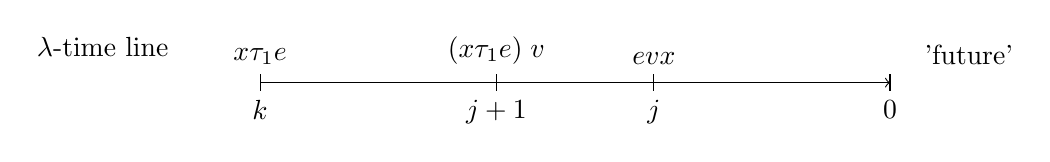
\begin{tikzpicture}
    % draw horizontal line   
    \draw[->] (0,0) -- (8,0);

    % draw vertical lines
    \foreach \x in {0,3,5,8}
      \draw (\x cm,3pt) -- (\x cm,-3pt);

    % draw nodes
    \draw (-2,0) node[below=3pt] {  } node[above=6pt] {$\lambda$-time line};
    \draw (0,0) node[below=3pt] {$k$} node[above=3pt] {$ \tlabs{x}{\tau_1}{e}$};
    \draw (3,0) node[below=3pt] {$ j+1 $} node[above=3pt] {$(\tlabs{x}{\tau_1}{e})\; v $};
    \draw (4.3,0) node[below=3pt] {$   $} node[above=3pt] {$ \evalto $};    
    \draw (5,0) node[below=3pt] {$ j $} node[above=3pt] {$ \sub{e}{v}{x} $};
    \draw (8,0) node[below=3pt] {$ 0 $} node[above=3pt] {$  $};
    \draw (9,0) node[below=3pt] {$   $} node[above=3pt] { 'future' };
  \end{tikzpicture}
\end{center}
Here we start at index $k$ and as we run the program we use up steps until we at some point reach 0 and run out of steps. At step $k$ we are looking at a lambda. A lambda is used by applying it, but it is not certain that the application will happen right away, as the we only do $\beta$-reduction when we try to apply a lambda to a value, but we might be looking at a context where we want to apply the lambda to an expressions, i.e.\ $(\tlabs{x}{\tau_1}{e})\; e_2$. We might use a bunch of steps to reduce $e_2$ down to a value, but we cannot say how many. So say that sometime in the future have fully evaluated $e_2$ to $v$ and say that we have $j+1$ steps left at this time, then we can do the $\beta$ reduction which gives us $\sub{e}{v}{x}$ at step $j$. % If we ever hit 0 steps, then all bets are off. the value can have any type.

We can now define the value interpretation of $\mu\alpha. \; \tau$:
\[
  \vpres{\mu\alpha.\; \tau} = \{\fold \; v \vbar \forall j < k. \; v \in \vpres[j]{\sub{\tau}{\mu\alpha.\;\tau}{\alpha}} \}
\]
This definition is like the one we previously proposed, but with a step-index. This definition is well-founded because $j$ is required to be \emph{strictly} less than $k$ and as we define the interpretation on induction over the step-index this is indeed well founded. We do not define a value interpretation for type variables $\alpha$, as we have no polymorphism yet. The only place we have a type variable at the moment is in $\mu\alpha. \; \tau$, but in the interpretation we close of the $\tau$ under the $\mu$, so we will never encounter a free type variable.

Finally, we define the expression interpretation:
\[
  \epres{\tau} = \{e \vbar \forall j < k. \; \forall e'. \; e \evaltos[j] e' \pand \irred(e') \; \implies \; e' \in \vpres[k-j]{\tau}\}
\]
To illustrate what is going on here consider the following time line: \\
\begin{center}
\begin{tikzpicture}
    % draw horizontal line   
    \draw[->] (0,0) -- (4,0);

    % draw vertical lines
    \foreach \x in {0,2,4}
      \draw (\x cm,3pt) -- (\x cm,-3pt);

    % draw nodes
    \draw (0,0) node[below=3pt] {$k$} node[above=3pt] {$e$};
    \draw (1,0) node[below=3pt] {$ $} node[above=3pt] {$\evalto \evalto \evalto \evalto$};
    \draw (2,0) node[below=3pt] {$k-j$} node[above=3pt] {$e'$};
    \draw (4,0) node[below=3pt] {$0$} node[above=3pt] {$  $};

    % brace
    \draw [decorate,decoration={brace,amplitude=10pt,mirror}]
    (0,-0.6) -- (2,-0.6) node [black,midway,yshift=-0.5cm] 
          {\footnotesize $j$};
\end{tikzpicture}
\end{center}
We start with an expression $e$, then we take $j$ steps and get to expression $e'$. At this point if $e'$ is irreducible, then we want it to belong to the value interpretation of $\tau$ for $j-k$ steps. The reason we use a strict inequality is that we do not want to hit 0 steps. If we hit 0 steps, then all bets are off.%TODO: why are all bets off?

We also need to lift the interpretation of type environments to step-indexing:
\begin{align*}
  \gpres{\mtenv} & = \{\emptyset \} \\
  \gpres{\Gamma, x : \tau} & = \{ \gamma[x \mapsto v] \vbar \gamma \in \gpres{\Gamma} \pand v \in \vpres{\tau} \}
\end{align*}

\[
  \Gamma \models e : \tau \eqdef \forall k \geq 0. \; \forall \gamma \in \gpres{\Gamma} \; \implies \gamma(e) \in \epres{\tau}
\]

\begin{stlcmufundprop}[Fundamental property] ~\\
  If $\Gamma \vdash e : \tau$ then $\Gamma \models e : \tau$.
\end{stlcmufundprop}
%TODO: something is missing here, write it.
\[
\circled{b} \quad \mtenv \models e : \tau \implies \safe(e)
\]

\begin{monotonicity}
  If $v\in \vpres{\tau}$ and $j \leq k$  then $v \in \vpres[j]{\tau}$.
\end{monotonicity}
\begin{proof}
We prove this by case on $\tau$.
\case{$\tau = bool$}
assume $v \in \vpres{bool}$ and $j \leq k$, we then need to show $v \in \vpres[j]{bool}$. As $v \in \vpres{bool}$ we know that either $v= \true$ or $v=\false$. If we assume $v=\true$, then we immediately get what we want to show, as $\true$ is in $\vpres[j]{bool}$ for any $j$. Likewise for the case $v=\false$.
\case{$\tau = \tarrow{\tau_1}{\tau_2}$}
assume $v \in \vpres{\tarrow{\tau_1}{\tau_2}}$ and $j \leq k$, we then need to show $v \in \vpres[j]{\tarrow{\tau_1}{\tau_2}}$. As $v$ is a member of $\vpres{\tarrow{\tau_1}{\tau_2}}$ we can conclude that $v = \tlabs{x}{\tau_1}{e}$ for some $e$. By definition of $v \in \vpres[j]{\tarrow{\tau_1}{\tau_2}}$ we need to show $\forall i \leq j. \forall v' \in \vpres[i]{\tau_1}.\; v' \in \epres[i]{\tau_2}$. Suppose $i \leq j$ and $v' \in \vpres[i]{\tau_1}$, we then need to show $v' \in \epres[i]{\tau_2}$.

By assumption we have $v \in \vpres{\tarrow{\tau_1}{\tau_2}}$ which gives us $\forall n \leq k. \forall v' \in \vpres[n]{\tau_1}.\; v' \in \epres[n]{\tau_2}$. From $j \leq k$ and $i \leq j$ we get $i \leq k$ by transitivity. We use this with $v' \in \vpres[i]{\tau_1}$ to get $v' \in \epres[i]{\tau_2}$ which is what we needed to show.
\case{$\tau = \mu \alpha.\; x$}
assume $v \in \vpres{\mu\alpha. \; \tau}$ and $j \leq k$, we then need to show $v \in \vpres[j]{\mu\alpha. \; \tau}$. From $v$'s assumed membership of the value interpretation of $\tau$ for $k$ steps we conclude that there must exist a $v'$ such that $v = \fold \; v'$. If we suppose $i<j$, then we need to show $v' \in \vpres[i]{\subst{\tau}{\mu\alpha.\; \tau}{\alpha}}$. From $i<j$ and $j \leq k$ we can conclude $i < k$ which we use with $\forall n < k.\; v' \in \vpres[n]{\subst{\tau}{\mu\alpha.\; \tau}{\alpha}}$, which we get from $v \in \vpres{\mu\alpha. \; \tau}$, to get $v' \in \vpres[i]{\subst{\tau}{\mu\alpha.\; \tau}{\alpha}}$.
\end{proof}
\begin{comment}
  \begin{lemma}[Substitution]
    Let $e$ be syntactically well-formed term, let $v$ be a closed value and let $\gamma$ be a substitution that map term variables to closed values, and let $x$ be a variable not in the domain of $\gamma$, then
    \[
    \extsub{\gamma}{x}{v}(e) = \subst{\gamma(e)}{x}{v}
    \]
  \end{lemma}
\end{comment}
\begin{proof}[Proof (Fundemental Property)]
Proof by induction over the typing derivation.
\case{\TFold} \\~
We need to show 
\newcommand{\mat}{\ensuremath{\mu\alpha.\tau}}
\[
  \Gamma \models \fold \; e : \mat
\]
So suppose we have $k \geq 0$ and $\gamma \in \gpres{\mat}$, then we need to show $\gamma(\fold\; e) \in \epres{\mat}$ which amounts to showing $\fold\; \gamma(e) \in \epres{\mat}$.

So suppose that $j<k$ and that $\fold\; \gamma(e) \evaltos[j] e'$ and $\irred(e')$, then we need to show $e' \in \vpres[k-j]{\mat}$. As we have assumes that $\fold\; \gamma(e)$ reduces down to something irreducible and the operationional semantics of this language are deterministic we know that $\gamma(e)$ must have evaluated down to something irreducible. We therefore know that $\gamma(e) \evaltos[j_1] e_1$ where $j_1 \leq j$ and $\irred(e_1)$.
Now we use our induction hypothesis:
\newcommand{\tsub}{\ensuremath{\sub{\tau}{\mat}{\alpha}}}
\[
  \Gamma \models e : \tsub
\]
We instantiate this with $k$ and $\gamma \in \gpres{\Gamma}$ to get $\gamma(e) \in \epres{\tsub}$. Which we then can instantiate with $j_1$ and $e_1$ for get $e_1 \in \vpres[k-j_1]{\tsub}$. Now let us take a step back and see what happend: We started with a $\fold\; \gamma(e)$ which took $j_1$ steps to $\fold\; e_1$. We have just shown that this $e_1$ is actually a value as it is in the value interpretation of $\vpres[k-j_1]{\tsub}$. To remind us $e_1$ is a value let us refer to it as $v_1$. We further know that $\fold\; \gamma(e)$ reduces to $e'$ in $j$ steps and that $e'$ was irreducible. $\fold\; v_1$ is also irreducible as it is a value and as our language is deterministic it must be the case that $e' = \fold\; v_1$ and thus $j = j_1$. Our proof obbligation was to show $e' = \fold \; v_1 \in \vpres[k-j]{\mat}$ to show this suppose we have $l < k-j$ (this also gives us $l < k-j_1$ as $j = j_1$). We then need to show $v_1 \in \vpres[l]{\tsub}$, we obtain this result from the monotonicity lemma using $\vpres[k-j_1]{\tsub}$ and $l < k-j_1$.
\end{proof}

The example with lists from the previous lecture used the sum type. Sums are a straight forward extension of the language. The extension of the value interpretation would be:
\[
  \vpres{\tau_1 + \tau_2} = \{\inl \; v_1 \vbar v_1 \in \vpres{\tau_1}\} \cup 
                            \{\inr \; v_2 \vbar v_2 \in \vpres{\tau_2}\}
\]
We can use $k$ directly or $k$ decremented by one. It depends on whether we want casing to take up a step. Either way the definition is well-founded. 

\subsection*{Universal Types}
Now we shift focus from type safety and termination to program equivalence. To motivate the need for arguing about program equivalence we first introduce universal types.

Say we want to implement a sort function. Maybe we even have a function that sorts integer lists:
\[
  sortint \; : \; \tarrow{list \; int}{list \; int}
\]
$sortint$ takes a list of integers and returns a sorted version of that list. Say we now want a function that sorts lists of strings, then instead of implementing a separate function we could factor the code and have just one function. The type signature of such a generic sort function is:
\[
  sort \; : \; \forall \alpha.\; \tarrow{(list \; \alpha) \times (\tarrow{\alpha \times \alpha}{bool} )}{list \; \alpha}
\]
$sort$ takes a type, a list of elements of this type, and a comparison that compares to elements of this type and returns a list sorted according to the comparison function. And example of an application of this function could be
\[
  sort \; [int] \; (3,5,7) \; <
\]
Whereas sort instantiated with the $string$ type, but given an integer list would not be a well typed instantiation.
\[
  sort \; [string] \; \cancelto{("a","c","b")}{(3,7,5)} \; string<
\]
Here the application with the list $(3,7,5)$ is not well typed, but if we instead use a list of strings, then it is well typed. 

We want to extend the simply typed lambda calculus with functions that abstract over types in the same way lambda abstractions, $\tlabs{x}{\tau}{e}$, abstract over terms. We do that by introducing a type abstraction:
\[
  \tLabs{e}
\]
This function abstracts over the type $\alpha$ which allows $e$ to depend on $\alpha$.

\subsubsection*{System F (Simply Typed Lambda Calculus With Universal Types)}
\begin{align*}
  \tau &::= \dots \vbar \forall \alpha. \; \tau \\
  e    &::= \dots \vbar \tLabs{e} \vbar e[\tau] \\
  v    &::= \dots \vbar \tLabs{e}\\
  E    &::= \dots \vbar E[\tau] 
\end{align*}
\[
  (\tLabs{e})[\tau] \evalto e[\tau/\alpha]
\]
Type environment\footnote{We do not annotate $\alpha$ with a kind, as we only have one kind in this language.}
\[
  \Delta ::= \mtenv \vbar \Delta,\; \alpha
\]
With the addition of type environments of type variables we our typing judgments now have the following form:
\[
  \Delta,\Gamma \vdash e : \tau
\]
We now need a notion of well-formed types. If $\tau$ is well formed with respect to $\Delta$, then we write:
\[
  \Delta \vdash \tau
\]
We do not include the formal rules here, but they amount to $\FTV(\tau) \subseteq \Delta$, where $\FTV(\tau)$ is the set of free type variables in $\tau$.

We further introduce a notion of well formed environments. An environment is well formed if all the types that appear in the range of $\Gamma$ are well formed.
\[
  \Delta \vdash \Gamma \eqdef \forall x \in \dom(\Gamma). \; \Delta \vdash \Gamma(x)
\]
For any type judgment $\Delta,\Gamma \vdash e : \tau$ we have as an invariant that $tau$ is well-formed in $\Delta$ and $\Gamma$ is well formed in $\Delta$. The old typing system extended with the new form of the typing judgment looks like this:
\[
  \FTFalse
\hspace{1cm}
  \FTTrue
\]
\[
  \FTVar
\hspace{1cm}
  \FTIf
\]  
\[
  \FTAbs 
\hspace{1cm}
  \FTApp
\]
Notice that the only thing that has changed is that $\Delta$ has been added to the environment in the judgments. We further extend the typing rules with the following two rules to account for our new language constructs:
\[
  \FTtAbs
\hspace{1cm}
  \FTtApp
\]
\subsubsection*{Properties of System-F}
In System-F certain types reveal the behaviour of the functions with that type. Let us consider terms with the type $\forall \alpha. \tarrow{\alpha}{\alpha}$. Recall from the motivation in lecture 1 that this had to be the identity function. We can now phrase this as a theorem:
\begin{theorem}
  If $\mtenv ; \mtenv \vdash e : \forall \alpha. \; \tarrow{\alpha}{\alpha}$,\\ $\mtenv \vdash \tau$, and\\ $\mtenv; \mtenv \vdash v : \tau$\\ then $e[\tau]\; v \evaltos v$
\end{theorem}
This is a free theorem in this language. Another free theorem that was mentioned in the motivation of lecture 1 was about expressions with type $\forall \alpha. \tarrow{\alpha}{bool}$. Here all expressions with this type had to be constant functions. We can also phrase this as a theorem
\begin{theorem}
  If $\mtenv \vdash \tau$, $\mtenv \vdash v_1 : \tau$, and $\mtenv \vdash v_1 : \tau$, then $\ctxeq{e[\tau] \; v_1}{e[\tau]\; v_2}$.
\end{theorem}
Or in a slightly more general fashion where we allow different types:
\begin{theorem}
  If $\mtenv \vdash \tau$, $\mtenv \vdash \tau'$, $\mtenv \vdash v_1 : \tau$, and $\mtenv \vdash v_1 : \tau'$, then $\ctxeq{e[\tau]\; v_1}{e[\tau']\; v_2}$.
\end{theorem}
\footnote{We have not yet defined $\ctxeq{}{}$ so for now just treat it as the two programs are equivalent without thinking too much about what equivalence means.}The reason we get these free theorems is that the function has no way of inspecting the argument as it does not know what type it is. As the function has to treat its argument as an unknown 'blob' it has no choice but to return the same value every time.

The question now is: ``how do we prove these free theorems?'' The two last theorems both talk about program equivalence which we prove using logical relations. The first theorem did not mention equivalence, but the proof technique of choice is still logical relations.

\subsection*{Contextual Equivalence}
To define a contextual equivalence we first define the notion of a program context. A program context is a complete program with exactly one hole in it. It is defined as follows:
\begin{align*}
  C ::= &\;  [\cdot] \\
        &\vbar \eif{C}{e}{e}  \\
        &\vbar \eif{e}{C}{e} \\
        &\vbar \eif{e}{e}{C} \\
        &\vbar \tlabs{x}{\tau}{C} \\
        &\vbar C \; e \\
        &\vbar e \; C \\
        &\vbar \tLabs{C} \\
        &\vbar C[\tau]
\end{align*}
We need a notion of context typing. For simplicity we just introduce it for simply typed lambda calculus. The context typing is written as:
\[
C:\; (\Gamma \vdash \tau) \implies (\Gamma' \vdash \tau') \implies \Gamma \vdash e : \tau \implies \Gamma' \vdash C[e] : \tau'
\]
This means that for any expression $e$ of type $\tau$ under $\Gamma$. If we embed it into $C$, then the type of the embedding is $\tau'$ under $\Gamma'$.

Informally we want contextual equivalence to say that no matter what program context we embed either of the two expressions in, it gives the same result. This is also called as observational equivalence as the program context is unable to observe any difference no matter what expression we embed in it. We can of course not plug anything into the hole, so we annotate the equivalence with the type of the hole which means that the two contextual equivalent expressions have to have that type.
\[
  \Delta; \Gamma \vdash \ctxeq{e_1}{e_2} : \tau \eqdef \forall C.\; (\Delta ; \Gamma \vdash \tau ) \implies (\mtenv ; \mtenv \vdash \tau') \implies (C[e_1] \Downarrow v \iff C[e_2] \Downarrow v)
\]
This definition assumes that $e_1$ and $e_2$ has type $\tau$ under the contexts specified.

Contextual equivalence is handy, because we want to be able to reason about the equivalence of two implementations. Say we have two implementations of a stack, one is implemented using an array the other using a list. If we can show that the two implementations are contextual equivalent, then we can use the more efficient one over the less efficient one and know that the complete program will behave the same.

In the next lecture we will introduce a logical relation such that
\[
  \Delta ; \Gamma \vdash \lreq{e_1}{e_2} : \tau \implies \text{contextual equivalence \ctxeq{}{}} 
\]
That is we want to show that the logical relation is sound with respect to contextual equivalence. 

If we can prove the above soundness, then we can state our free theorems with $\lreq{}{}$ rather than $\ctxeq{}{}$ and get the same result, if we can prove the logical equivalence. We would like to do this as it is difficult to directly prove two things are contextual equivalent. A direct proof has to talk about all possible program contexts which we could do using induction, but the lambda-abstraction case turns out to be difficult. This motivates the use of other proof methods where logical relations is one of them.

\subsection*{Exercises}
\begin{enumerate}
\item Do the lambda and application case of the \emph{Fundamental Property} theorem.%Specify in what proof, probably fundemental property
\item Try to prove the monotonicity lemma where the definition of the value interpretation has been adjusted with:
\[
\vpres{\tarrow{\tau_1}{\tau_2}} = \{\tlabs{x}{\tau_1}{e} \vbar \; \forall v \in \vpres{\tau_1}. \; \sub{e}{v}{x} \in \epres{\tau_2} \}
\]
This will fail, but it is instructive to see how it fails.
\end{enumerate}


%induction on step index followed by inner induction on the type structure.
%when an expression looks like it has type tau.
\clearpage
